%\addcontentsline{toc}{chapter}{Development Process}
\chapter{Design}

This chapter describes the design stage of developing Location Sensitive Social Notifier and it also covers in depth the final design that was implemented in the final version of the application.

\section{Overview of architecture}

This section will cover the design of the applications at key stages of development, covering the initial design at the beginning of the project and how it matured to the version that we have today. This section will also cover the future development that will needed to be done to make the application a viable fully fledged application that can be released to the general public.

\subsection{Initial Design}
\label{sec:global_initial_design}

\subsubsection*{Background}

As the project was done in a iterative and evolutionary style of development there was not much up front planning in the way of initial design. I sketched out a few initial ideas of the block design of the application with all the major parts of the framework including front end, middle tier and database, without any fine details.
The original plan was to use an Oracle APEX backend which would handle all of the REST requests and SQL side of things, but due to licensing and the fact I wanted to learn new technologies this idea fell by the wayside and it was decided to try and use a middle-ware along with a SQL database. \\
\\
It was unclear at the start of the project what platform the application would be developed for, with the choice being between Apple iOS, Google Android or Phone Gapp. So in the early design this left some ambiguity as to how various features and UI design should be implemented. This means in early diagrams the design is very generic and not platform specific.
Theses early sketches were devised from the ideas that had been formulating since I had first envisioned the idea the previous year. The next step was to break the application as a whole and break it down into its functional requirements.

\begin{figure}[H]
    \centering
    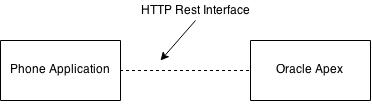
\includegraphics[width=0.5\textwidth]{diagrams/initialblockdiagram}
    \caption{Original design of the application}
    \label{fig:apex_block_diagram_image}
\end{figure} 

\subsubsection*{Functionality}
\label{sec:functionality}

Assessing the functional requirements required breaking down the concept into its core components. Most noticeably posting, viewing and being notified about tags were the core functionality for the application. Without these features the application could not achieve the goals set out in the original specification, thus undermining the usefulness of the finished application.\\
\\
Viewing a message that is left in the application is a core part of the functionality that is required by the application. It should be very easy and uncomplicated for the user to view a tag that has been left by their friends. The application's overall success will most possibly rest on the speed of viewing a message and quickly being able to leave feedback on the tag that has been left. The UI should be easy to interpret with the minimal UI on the screen to ensure that there is no confusion in the message that is trying to be conveyed. A simple and minimal UI also gives the application an attractive aesthetic that should mean that users are attracted to using the application. It should be easy for the user to decide if the tag is publicly available or limited to friends to ensure the flexibility of the application.\\
\\
An equally important feature that makes the application is the posting of messages. Without the ability to post a message the application is a void concept and generally to view messages there needs to be the ability to post messages. Again the key aim of the application is to make it easy to leave messages without any extra complexity that might discourage the user from leaving a message. The UI should be as minimal as possible while portraying the intent of the screen in a simple and straight forward way. Some clever UI design should help draw the interest into the page and enable the user to understand what is happening. The use of a map fragment on this page to show where the user is when they post their message is a good way to draw attention into the posting of a message. The user should be able to enter a message of a reasonable length into the fields within the application.\\
\\
The final core functionality that is integral to get the application to work as desired is the notification portion which notifies the user of the tags that are near by to the user. This should run with no input from the user and should quickly and efficiently provide the user information about the nearby tag. When the user interacts with the notification then they should be able to quickly and effectively navigate to the view message page. They will not have to go into the application itself to select this but the notification will automatically take the user to the view message screen for them to interpret what the message is.\\
\\
More minor functionality is dealing with friends within the application, so adding the user's friends so that they can interact with them within the application. Adding friends to their account should be straightforward with a search that enables them to find and add them to their account. This should also not be a cluttered page with the bare minimum UI elements to get the job done correctly as this should minimise the confusion from using the application and means it should be more likely that users user the application and recommend it on to their friends to actually use it. Continuation of the friends theme is that it should be very easy for users to add viability to messages for their friends to view it. Giving a user viability should mean that they will get notified of the message when they are close by to it.\\
\\
The application will also require having some operations for dealing with authentication with the server. So it is essential for the application to have screens to register and login to these screens should be as simple as possible, only asking the true essentials to get the job done, with clear and simple forms that will not lead to confusion and frustration that would lead to them being put off using the application. Keeping the forms simple should also improve security as it's less fields to protect from attack and thus being compromised by a potential malicious user.

\subsubsection*{UI mock-ups}

Once the application had been broken down into the various functional areas I started to do some rough user interface layouts on paper. Once they were to a satisfactory level they were converted into digital mock-ups using Balsamiq which created the figures \ref{fig:application_home_page_image}, \ref{fig:add_friend_activity_image}, \ref{fig:add_tag_activity_image}, \ref{fig:viewing_message_image}, \ref{fig:giving_friends_visability_image}, \ref{fig:login_activity_image}, \ref{fig:registration_activity_image} and \ref{fig:notification_image}. \\
\\
The UI design takes some inspiration from other phone applications, in particular Snap Chat with the way of quickly sharing messages and Facebook with the quickly accessible stacked menus. The main reason I took inspiration from Snap Chat is because their application is very quick to use and post messages and the general concept of Lo Se Sono is almost the same bar and locations are used rather than pictures and there is no set timeout on the tags.\\
\\
At the time of creating the mock ups it was not clear for which platform the application was going to be implemented, so the designs have remained very generic without being OS specific.\\
\\
These UI mock-ups were used to create the final application. The designs may have been slightly modified between the original design and the final implementation within the application.\\
\\
Figure \ref{fig:application_home_page_image} is the design for the main page of the application and where the users arrive when the application launches, so it is of utmost importance that this page is easy to navigate and informative to the user. The UI has been intentionally designed to show the tags that are most relevant to the user at the time they have opened the application, showing the tags in their immediate vicinity. These can be either the user's own tags or their friends who have left them there.\\

\begin{figure}[H]
    \centering
    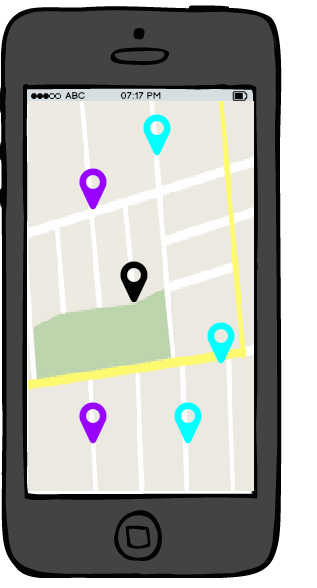
\includegraphics[width=0.25\textwidth]{uimockups/homepage}
    \caption{Application home page}
    \label{fig:application_home_page_image}
\end{figure}

\noindent
In figure \ref{fig:add_tag_activity_image} we are showing the initial design for adding a tag to the map. The key idea is to make it quick and easy to add a tag to the map and make it quickly accessible to the user's friends so they can be promptly notified about the tag their friend has added.\\

\begin{figure}[H]
    \centering
    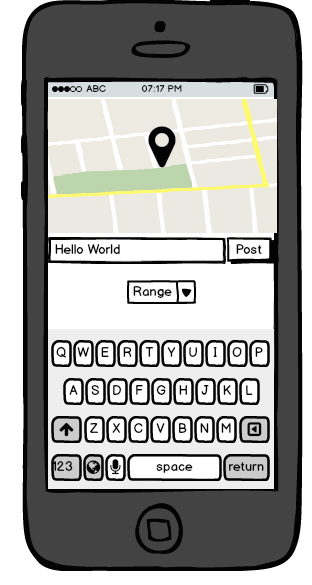
\includegraphics[width=0.25\textwidth]{uimockups/addtag}
    \caption{Adding a tag activity}
    \label{fig:add_tag_activity_image}
\end{figure}

\noindent
Pictured in figure \ref{fig:giving_friends_visability_image} is the screen that enables user's friends to view a message that has been left. It should be relatively straight forward and easy to interpret. The design has changed ever so slightly in the final implementation to try and make it fit in better with the Android design principles.\\

\begin{figure}[H]
    \centering
    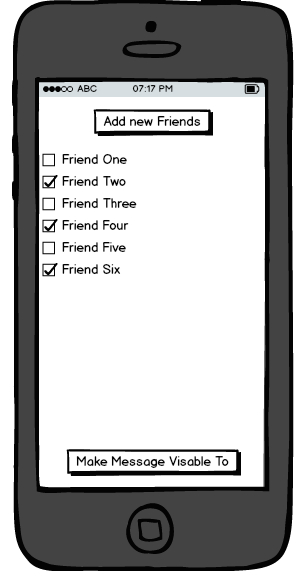
\includegraphics[width=0.25\textwidth]{uimockups/friendsvisability}
    \caption{Giving friends ability to view message}
    \label{fig:giving_friends_visability_image}
\end{figure} 

\noindent
This is the UI in figure \ref{fig:add_friend_activity_image}. To add a new user to the user's friends list it gives the user the ability to search for their friends using their names. In the final version of the application the search functionality remains unfinished within the UI, but was partially completed within the server side application. When this functionality is implemented it should make it very easy for the user to add new friends within the application, thus expanding the audience of the application.\\

\begin{figure}[H]
    \centering
    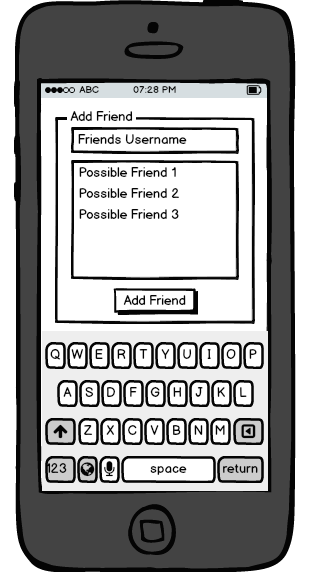
\includegraphics[width=0.25\textwidth]{uimockups/addfriend}
    \caption{Adding Friend activity}
    \label{fig:add_friend_activity_image}
\end{figure} 

\noindent
This figure \ref{fig:viewing_message_image} shows the viewing of a message. This is the screen that has changed the most from the original UI mock ups, where the icons and location of the voting section has been moved to be above the commenting area. There is also now a fixed area at the bottom for adding a comment, along with each comment section now including their own voting sections. But again the changes to the initial designs have intentionally been very minor.\\

\begin{figure}[H]
    \centering
    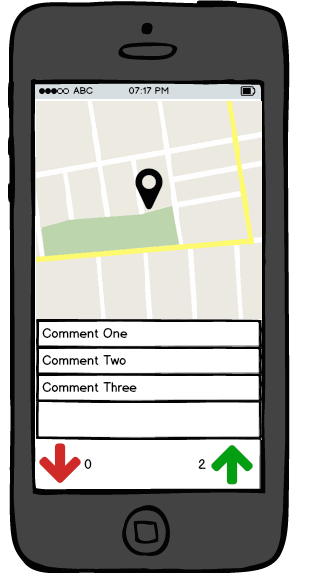
\includegraphics[width=0.25\textwidth]{uimockups/viewmessage}
    \caption{Viewing a message}
    \label{fig:viewing_message_image}
\end{figure} 

\noindent
The image below in figure \ref{fig:login_activity_image} shows the login screen for the application. This was intentionally kept simplistic to ensure that it is easy for the user to interpret and should make it fairly secure against attacks as there are less fields to attack.\\

\begin{figure}[H]
    \centering
    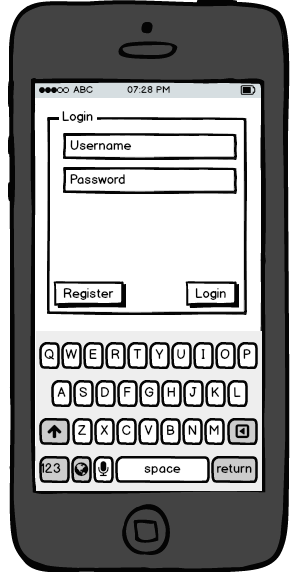
\includegraphics[width=0.25\textwidth]{uimockups/login}
    \caption{Login Activity for the application}
    \label{fig:login_activity_image}
\end{figure} 

\noindent
Screenshot pictured in figure \ref{fig:registration_activity_image} describes the registration page within the application that enables the user to register to use the application. Again it has been kept simple to avoid confusion and ensure that the user can navigate it easily. This should ease annoyance when people are using the application for the first time.\\

\begin{figure}[H]
    \centering
    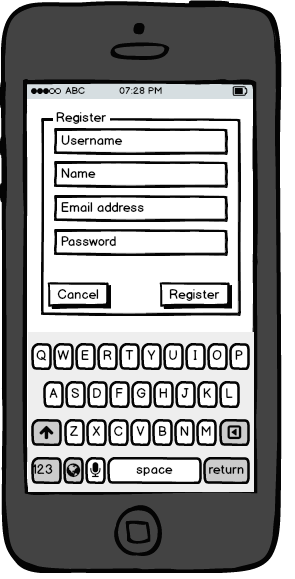
\includegraphics[width=0.25\textwidth]{uimockups/register}
    \caption{This is the activity for registering to use the application}
    \label{fig:registration_activity_image}
\end{figure} 

\noindent
This screenshot in figure \ref{fig:notification_image} is an example notification for the application. In the final application this does not look anything like this due to the fact we are using the Google Android notification API and notifications do not appear in this way.\\

\begin{figure}[H]
    \centering
    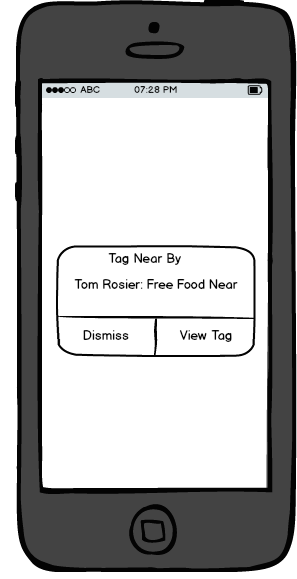
\includegraphics[width=0.25\textwidth]{uimockups/notification}
    \caption{Notification that there is a tag near by}
    \label{fig:notification_image}
\end{figure} 

\noindent
These designs were used as reference to build the applications UI for the final design. They have intentionally kept similar to the original mock-ups as it was felt that the designs would be easy for users to interpret and a good starting point.

\subsection{Final Implementation}

As the project was developed in an eXtream programing style there was not much design done up front. The major design that was done up front was a list of the main functionality within the application and the final implementation of those features were done in an iterative form. There was a very initial block diagram done showing the different main sections of the application, which is shown in figure \ref{fig:initial_diagram_image}. This is the basic design of the application without any of the specifics, e.g not detailing the libraries that have been used to implement the full application.\\

\begin{figure}[H]
    \centering
    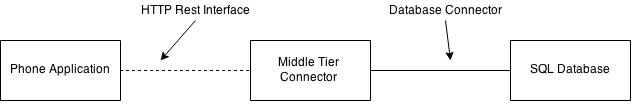
\includegraphics[width=\textwidth]{diagrams/blockdiagram}
    \caption{Very simple block diagram from the start of development}
    \label{fig:initial_diagram_image}
\end{figure} 

\noindent
The final implementation started with spike work into different frameworks that could be used for the development of the project. I started with the Phone side of the application where there was research into whether to use Phone Gapp or to go for a native application. The reasoning and decision to use an exclusively Google Android are covered in section '\ref{sec:android_choice_of_tech} Choice of technologies'.\\
\\
Next the focus moved onto the server side application. The choice of server side environment was focused on looking at cutting edge but also fairly mature server side platforms. The choice was between Node.js with express, Node.js with HAPI.js, Node.js with StrongLoop, Python Flask or Java TomCat. Please refer to '\ref{sec:node_choice_of_tech} Choice of technologies' for more in detail discussion about the rational between the choice of server side frameworks.\\
\\
Finally the decision turned to how the data would be stored within the application. The first decision was between a SQL or NOSQL solution. After some consideration it was decided that even though NOSQL is an interesting new area, it would be best to stick with the skills already learned as taking on too many new frameworks could compromise the success of the project. The final decision was to choose between what type of SQL engine to use to hold and process the data within the application. The decision was between PostgresSQL, My-SQL and SQLite. The pro's and con's are covered in detail in section '\ref{sec:database_choice_of_tech} Choice of technologies'.\\
\\
The diagram in figure \ref{fig:final_block_diagram_image} shows the finished architecture with the joins between each different technology that is needed to make the application work correctly and as desired in the way decided within the functional requirements. It is fairly obvious from the diagram that the application requires a lot of 3rd party libraries to work as intended, heavily relying on the Google Maps API, Android Asynchronous HTTP Client API, HAPI.js \& Sequelize to provide the major components within the project.\\

\begin{figure}[H]
    \centering
    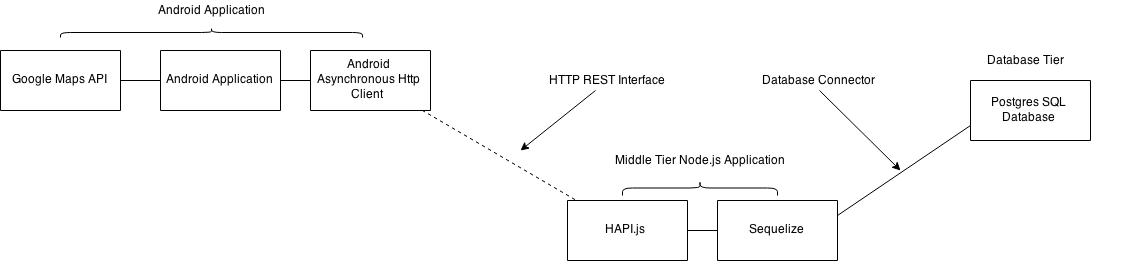
\includegraphics[width=\textwidth]{diagrams/finalblockdiagram}
    \caption{Very simple block diagram of the final architecture}
    \label{fig:final_block_diagram_image}
\end{figure}

\noindent
Standing on the shoulders of giants springs to mind as it would not be possible without all of these 3rd party libraries for the application to work in a usable and robust manner. Even with the use of all these 3rd party libraries there is still a fair bit of custom code to act as an aggregate for all the various parts of the functionality within the project together. The core functionally of the application is complete, but I would currently classify the application as a proof of concept due to the fact the robustness of the application and stability are currently questionable. How these issues will be overcome in the future will be covered in section \ref{sec:development_future_dev}.

\subsection{Future Development}
\label{sec:development_future_dev}

Due to the time constraints and time line of the project it was only possible to complete the application to a proof of concept stage. This section aims to cover the development that would need to take place to make the application viable for release into the consumer space. Firstly the current prototype does not have any consideration taken for preserving power. With the current prototype it very rapidly drains the battery of the devices that it is on and leads to the phone being critically low on battery after a few hours. This will be resolved in further development, which would be more intelligent about when it turns on the GPS, and will use the accelerometers in the phone to gauge if it has moved any considerable distance since the GPS was last turned on and then also changing the duration between the checks to ensure that the phone hasn't moved very often would mean that the duration that we check should decrease, thus helping save the battery on the phone. But in cases where the phone is constantly on the move it is very likely that application will remain very high power due to the nature of GPS. Some effort can be put into the wastage as well if the device can't get a fix, then we should not keep trying as this just drains the battery.\\
\\
Again due to time constraints and how large the catalogue of devices are within Android, there has been limited optimisation of the getting the UI to work perfectly on all devices. Also for the development stage the application has only been designed \& tested on a 1080p device due to being the main device that I had access to, but with more time more consideration and multiple layouts could be made to make the application scale and work correctly on different sized devices.\\
\\
The other point that needs to be raised is due to it being a proof of concept. The application does not fail gracefully and an exception in how the application is used will cause the whole thing to come crashing down around itself without giving any dialog to the user about what has happened. Before the application can be released into the consumer marketplace it will need to have the error catching and handling clearly and robustly implemented so the application can handle any unusual events or unexpected situation. Along with this it is advised to create a full testing suite for the application to ensure that any changes made within the application do not break the whole application and that the operations all complete in the way that they are intended to complete.\\
\\
With theses changes I can see the application being a well used and popular application that will make it an interesting concept that people will pickup and use. I would not consider releasing the application until these changes have been done, as it would not reflect well on the developers to have these issues within the early releases of the code.

\section{Client Side}

%Alison got to here.

The client side part of the application is the part that user actually sees and interacts with, for this project it was elected to use a Google Android phone application to be the main focus for the end user. It needs to act as a way to draw users into using the concept and illustrating the benefits of the ideas behind the application as a whole, it needs to be robust and usable for it to gain wide adoption within the consumer space. If users find the application fun and easy to use it is highly likely they will recommend the application to there friends and it will gain widespread adoption within the popular culture which would be a ideal situation and would mean that project has been successful.

\subsection{Why A Android Application}

Android is a cutting edge mobile platform that is used by many millions of people it is statistically speaking the most popular mobile platform out there with over 50\% market cover \cite{statista:devicestats:2015:online}. To get near blanket market coverage it would be best to develop for Apple iOS as well as it has a market share of over 40\% but due to the time constraints of the project it is only possible to target one of theses platforms, due to have a multitude of Android devices close to hand it only seemed sensible to develop for Android over its competitors, for more detailed explanation of why the choice was to use Android refer to this section \ref{sec:android_choice_of_tech}.\\
\\
Android has is a very diverse selection of devices it will run on, as Google does not limit what devices that it can be run on so any hardware manufacture can decide to create an Android device meaning that they can vary massively between devices there is almost an infinite array of screen sizes and screen resolutions that Android will run on along with a large array of different processors that it will run on due in part to Androids open sourced routes and its deep origins from Linux it gives it a very strong versatility and this means its very popular with the computer science community and users that like to tinker. Although one of the main drawbacks to Android is that ecosystem is fairly fragmented with many different versions of the operating system out in the public domain which means its difficult to get applications developed on Android to work on all of the devices out in the public domain either due to there form factors or due to the fact they are running a out dated version of the operating system which leads to incomparability with the newer code libraries. Luckily 93\% of devices \cite{google:osstats:2015:online} out in the wild are running fairly recent versions with the majority of theses devices running a API level between 15 and 22 which means that most code will run on the majority of devices as long as the developer is not seeking the most bleeding edge API's for there application.\\
\\
For this project it was decided to target the application at API level 14 which is known as 'Ice Cream Sandwich' and higher as this would give the ability to use fairly recent API's but also covering the mass majority of the devices out in the wild. API level 14 dates back to 2011 with the launch of Android 4.0 which means that we can support nearly all devices that were released in the last 5 years as flag ship phones from 2009 \& 2010 are fairly likely to still receive updates to 'Ice Create Sandwich'. Due to the user community that goes with Android it is fairly likely that theses old devices will have been updated via 3rd parties to run newer versions of Android than the original manufactures intended.\\
\\
The Android developers hub provides a very comprehensive set of API documentation along with tutorials on how to develop for Android with best practice documentation on the best way to design the application to make it fit in with the style of the Android ecosystem, some of the early research done for the project was based on reading the Android material design manual to ensure the application had a consistent theme and would be accessible to all sorts of different devices and users which would ultimately help with the adoption and usability of the final application.

\subsection{Choice of Technologies}
\label{sec:android_choice_of_tech}

The spike work / research that was carried out in the design stage started out by reading about the development experiences of various teams Phone Gapp vs Native to develop there various phone application and the reviews that I got seemed to be very mixed they ranged from saying to avoid or this is the best thing ever, with no clear way to move forward it the next stage was to research the API's that would be essential to the application working this being the Mapping API's and the GPS location. It quickly came apparent although Phone Gapp its fairly mature it could not compare to the libraries that were offered by the native solution.\\
\\
One of the benefits of using Phone Gapp over native is that it uses standard web technologies for example HTML, JavaScript \& CSS which I as the developer already knew fairly well and would not need to learn a new language to work on the application but this would still require learning a new framework to work on the application. Another benefit of using Phone Gapp is that the application will run on a multitude of devices from Apple iOS, Google Android and Microsoft Windows Phone where as choosing to go native means that application will only work on the framework and device it is programmed for.\\
\\
One of the major downsides of using Phone Gapp is that if there is not a library that exists for a given problem within the application then the developer is required to write in native code a library to couple the Phone Gapp application to the function provided by the phone. Due to this it was decided it would be best to just develop the application in native code as it eliminates theses coupling issues if they do arise. Along with the extra performance given by running within the native framework and not having another interpretive layer between the user and the phones hardware gives the developer and ultimately a better experience with the application.\\
\\
It was clear the best way forward was to use native development, my choice was then limited by what hardware that I already owned and due to only owning a Android based phone the decision was essentially made up for me and thus the development of a native Android application was the way forward, the major downside of developing for Android that although it is the majority platform out there, Android users tend to be less engaged with the application community than iOS users meaning that the adoption would be potentially hurt by deciding to target Android first. In the commercial work it is very likely that developers will create a native application for both Android and iOS to make sure there is adoption on the two main smart device platforms thus leading to near blanket coverage of the market.\\
\\
For the choice in Mapping API's there was only two solutions using official Google Maps API or Nutiteq Maps SDK, after some consideration it was apparent that Nutiteq was not as mature or well supported as the official Google Maps but did offer some nice additional features that the Google Maps API did not like the ability to have offline maps and the use of custom perspectives. It was decided to use the Google Mapping API as it had a mature community and is well supported, but if the decision was made at the end of the project the use of the Nutiteq API may have been a better choice due to the very limited and outdated documentation for the Google API which was a big disappointment.\\
\\
For dealing with rest requests it was decided to use Asynchronous HTTP Client for Android \cite{nknj:AndroidAsynchronousHttpClientloopjandthePersistentCookieStore:2013:online} as this was a well documented API with all the functionality that was needed to deal with all of the requests that needed to be carried out within the application, it gives a good flexibility for processing JSON objects that are returned from the server along with doing it all asynchronously to which will improve the snappiness of the application while dealing with requests.\\
\\
The interaction between the server and the Android Application is provided by an HTTP RESTful interface which enables robust and reliable standard for sending transmitting data, the ability to send JSON objects directly back and forth between the server and client makes data manipulation easy and means that the interface between the client and server is not platform or language specific which means it should be easy to add in another client that can use the API provided by for the application.

\subsection{Initial Design}

As mentioned previously the application was developed in a evolutionary way, with functionality only being added when it was essential to proceed with the application this mean there was not much in the way of up front design. For the Android side of the application the the way in upfront of design was to create a list of the functional requirements of the application detailing what the application needed to achieve to be a successful project these theses are listed within section \ref{sec:global_initial_design} and was mostly orientated towards the UI design of the application rather than the background architecture the architecture will be covered in detail in section \ref{sec:android_application_structure}.\\
\\
In the early thoughts about the layout and design of the application it was apparent that a model view controller approach should be taken to the design of each parts of the application, meaning that data structures, and viewing of the data are segregated out and there is a interconnecting layer between them to create a structure that is decoupled meaning that code is not written specifically to do one job and can be reused in many places to do many jobs which simplifies duplicated code and should ensure that code only has to be debugged in one place and is not copied to multiple locations throughout the application which should ensure that bugs are not encroached into the code base which could compromise the robustness of the application as a whole.\\
\\
Most of the initial design for the application was to investigate the frameworks that would be used within the application ensuring that they would suite the functionality requirements for the application, at first it was fairly hard to find a well documented and robust framework for dealing with HTTP requests to the background services to get the information that will be displayed within the application. The first framework that was tried seemed to have some stability issues and deal with all requests synchronously which mean the application would stutter while trying to retrieve data along with having stability issues which made the application unstable in real world operations. Another chunk of the early design stage was trying to get the Google Maps API to respond in a way that was usable for the needs of the project, which included the ability to tag locations and show robust labeling with the custom messages left by the user.

\subsection{Application Structure}
\label{sec:android_application_structure}

The structure of the application is based around it activities which is Android's name for screens, each activity has its own job to fill a place within the functional requirements of the application theses requirements can be found in section \ref{sec:functionality}. Usually it is a activity for each of the function so for example creating a new tag would have its own activity with its own supporting classes. An example of how the code is structured for each of the activities can be seen in figure \ref{fig:activity_interation_image}, data flows two and from the screens back and forth to the rest client part of the application that deals with interaction with the server either retrieving or sending data back to enable the functionality within the application.\\

\begin{figure}[H]
    \centering
    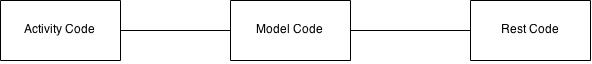
\includegraphics[width=\textwidth]{diagrams/activityinteraction}
    \caption{This is the simplified interaction between activities}
    \label{fig:activity_interation_image}
\end{figure} 

\noindent
Model and RESTful client layers of the structure are shared between larger parts of the functionality and may encapsulate everything to do with for example sending and receiving messages, along with all the other permutation of this format being contained within the same class to group them together functionality and make them easy to access and work with. They have tried to be kept as uniform and repetition kept to a bare minimum which should help with creating a easy to work on easy to maintain application that is an enjoyable code base to work on.\\
\\
The main point of entry for the application is the Navigation Activity which is the screen that shows all of the tags that are close by to the current user and there relevant to them, all of the application is ran from this point from this screen it is possible to reach all of the other activities and is the home page that the users land on when the execution begins it is the focal point of the application and is a return point after every operation has finished.\\
\\
There are other services that are run along side the activities one example of this is the notification service that enables the user to receive notifications that are relevant to them without viewing the application, they are push notifications the end user can view outside of the application and they add an extra bit to the user experience of the application.

\subsection{Caveats}

This section is dedicated to some of the shortcoming in the design of the Android Application and explanation of the issues. As Fred Brooks said in the Mythical Man Month \cite{fredbrooks:throwoneaway:1995:online} "Plan to throw one away; you will anyway" and it is fairly true in this situation, developing a application in a totally new framework to the developer means that some of the design choices can be misguided which results in the applications overall stability and design being hurt. Overall the design of the application as a whole is not bad but there are places where it is a little patchy and not designed to the best standard.\\
\\
The application will need some refactoring and design tweaking to make it a rewarding code base to work on as it stands if more functionality was added to some of the activities it would quickly become very difficult to work on with Spagetti code being the only way forward to patch on the new functionality. This will ultimately lead to a bad customer experience which will alienate users of the application and make them not want to use the application which would kill any representation that the application gains.\\
\\
As mentioned previously the fact that the application is only available for Android means that the audience for the application is limited to only half of the potential users out in the world due to the other users using Apple iOS, As part of the further development of the application it would be advised to develop an Apple iOS version of the application or scrap the current code base and move to Phone Gapp based application which would mean the application will work on any of the major smart phone operating systems.\\
\\
More research could of been done in implementing the various background services that are used within the application as they are in the version included with this a bit temperamental, this is somewhat down to the very limited documentation offered by Google on how to implement features that have provided by the Android Operating System its self. This was also not aided by the fact that some of the documentation for the various API's most notably the Google Maps API is heavily out of date and will not actually work on the device with the instructions given in the API documentation.

\section{Server Side}

The server side of the application is the part of the user does not directly interact with and handles the underlying functions behind the application working correctly this functionality gives an underlying service that enables the usability of the application. Theses services are responsible for supporting the RESTful interface between the application and back end, along with providing coupling between the RESTful interface and the database.\\
\\
The back end services are there to provide an effective data store for the users information along with providing the layer to create the interaction between users as the data is stored and processed on the server verses all the information being stored on the clients devices which would lead to the application being unmanageable due to data being placed in multiple different places along with when a device is offline then the data is unaccessible to other users.\\

\subsection{Middle Tier}

The middle tier is the connective tissue of the application acting as a intermediary between the database and the front end application. Its main purpose is to act as a HTTP server along with a client authentication point to ensure that only registered users can use the application. It is connected to a PostgresSQL database which handles storing data in a persistent form which can be easily interacted and manipulated to archive the desired functionality within the application that the end user can see and gives the application the desired effect.\\
\\
For this important task it was decided to use enterprise level frameworks and technologies, it was integral that the platform and the frameworks that were used to provide the functionality were robust, flexible and easy to work with I concluded to use Node.js \cite{nodeteam:node:2015:online} with the HAPI.js \cite{hapiteam:hapti:2015:online} was the best route to go down as it is fairly cutting edge but also has big supporters and a good support community, HAPI.js provided a robust and usable framework that was not overly complicated for the scenario that it would be used. It was also felt that the platform that the system is run on is not platform specific and can be run on any of the three main operating systems, thus the background services although have not been tested theoretically will run on a Linux Server along with an Apple OSX Server and Windows Server which means that if a platform change was needed in the future it should be easily possible to move the application's backend over to a different platform. More in depth reasons to why theses platforms / frameworks were chosen can be found in \ref{sec:node_choice_of_tech}.\\
\\
The user of a HTTP RESTful interface between the middle tier and the Android application seemed the most modern and best way of providing an link between the client and the background API that handles the data for the users of the application, it is also not platform specific which means it should be possible to add in other platforms that use the service at later points which can make use of the platform that already exists. This also translates over to the backend of the application because if the backend was ever replaced with another platform and services as long as the API end points returned the same data and the authentication worked in the same way then any client side application will work in the same way and the users would not see any different in the service.\\
\\
For the design of the backend application it was key to make it as modular as possible to ensure that it is fairly easy to add new functionality in as it was decided it would be best to use dynamic loading where possible, the application takes a list of route files which are for each part of the functionality given for the application for example there may be a route dedicated to all things messaging and if there was a need for a new bit of functionality not seen at the start of development then another route can be loaded in to add functionality needed within the backend application to handle the new functional requirement without the need to redesign the whole application and potentially damage the integrate of the application.\\
\\
Initial design for the backend of the application was to create a list of the corresponding RESTful endpoints for the functionality provided by the Android application, as the project progressed some alterations were made to this initial list for unforeseen functionality changes for example segregating the users messages from the friends messages and not have them all in one rest endpoint.\\
\\
The backend is linked to the database through a database connector the one that has been used is called Sequelize \cite{SaschaDepold:Sequelize:2015:online} and provides a Object Relational Mapping(ORM) which was originally going to be used within the application but it was quickly decided to use the raw SQL functions provided by the connector. The ORM functionality may be implemented properly at some point in the future development of the application and it was personal preference to elect to use the raw SQL interface as it was what I was more comfortable with and allowed better control over the data that was being returned from the database. Sequelize had one very nice feature that meant that JSON objects could be returned directly from the database which in some cases can be sent straight to the front end application without modification, which helps reduce the complexity within the application as a whole and makes it easier to debug in the long run.

\subsubsection*{Choice of Technologies}
\label{sec:node_choice_of_tech}

There were many different choices that could of been made for the platform and framework to run the back end application on, the 4 major platforms that it came to decide from was Java, PHP, Python and Node.js. Java was quickly ruled out as it was felt that it was to heavy weight and clunky for the application although it would be a better choice if the application became a heavy weight enterprise level application, Oracle offer very good support for Java based applications with very comprehensive API documentation along with the fact that the Android Side is developed in Java meaning there would only be one programming language for the whole project reducing the learning for the project as a whole but it was felt it would not be a good fit for the project. Next the attention was turned to PHP, PHP is a well known language for doing web based API's and is a long standing contender for doing this type of work my prior experience of PHP had not been very rewarding experience and it was a horrible language to work with which instantly gave me concerns to where it stands within this project along with some reports floating around at the time of starting the project about serious security issues PHP was dead in the water.\\
\\
This is where things get a bit more interesting the choice between Python and Node.js was very close due to the fact that they are up coming platforms with strong enterprise level functions along with being very powerful dynamically typed languages which enables high flexibility with how the application is designed. Both of the platform have very good frameworks to enable robust and clever web frameworks which would be perfect for this project along with very mature automated installation tools for the extra libraries that would be needed to run the software with Pythons PIP and Node.js's NPM tools making the portability of the applications much better solution than the PHP and Java alternatives. Ultimately the choice between the two platforms was made on what I as the developer already knew Python nearly won the battle but due to already knowing Node.js and the fact I would have to relearn Java and Android it was decided that learning 2 new languages may be a tall order and would be likely enough to jeopardise the project as a whole this was not a risk that I wanted to take.\\
\\
After deciding that Node.js was the way forward the next major decision was to choose what framework to use to build up the web services there was quite a few choices for this Express.js, Restify, HAPI.js and StrongLoop. Some of the reasoning came from the blog post by Alex Gorbatchev \cite{AlexGorbatchev:CompairingExpressRestifyHapLoopBack:2015:online} but I felt it was a little bit skewed by the fact it looked like he was a developer for StrongLoop along with the page being hosted on there blog. Restify was the first to be looked at as it promised the ease of creating simple restful services and strongly advertised it was intended for API's rather than websites, but after some close investigation it was felt that it was to restrictive and didn't have much support from large organisations and looking closer into support there did not seem to have a large community behind it. Next the attention was turned to Express.js which on the surface looked like it would most likely be the framework choosen for the application I had previously used Express.js and had enjoyed working with it, it is also robust, well tested, well proven but the only negative that can be said about it is that it is aimed more towards browser based web applications which is not what is desired for the project I am 100\% sure that Express.js could of been the de facto framework used within the project but I felt like a challenge and wanted to use something new.\\
\\
Next we will talk about the two frameworks that were in the top two, after throwing out Express.js my attention was drawn to StrongLoop after browsing there API documentation and marveling how clean and pretty the code looked I was pretty set on using it, I setup a development environment for the framework and immediately hit a brick wall with the learning curb presented by StrongLoop. StrongLoop is a Model View Control(MVC) based framework and requires lots of configuration to work correctly and relies on Object Relation Mapping to interact with its database. After couple days of going know-where it was best to reassess the decision after finding that the strict MVC to restrictive getting in the way of getting work actually completed the conclusion was to re-investigate the option at this point HAPI.js popped up as an option after further some investigation. HAPI.js seemed to have everything going for it it had big name supporters Disney, Yahoo, PayPal, Mozilla and Walmart just to name a few along with a strong development community and very useful Internet Relay Chat channel that could be used when extra support was needed. With some small spike work it was clear to see that HAPI.js with its simple but very powerful API was the way forward, within a few hours the progress with HAPI.js was impressive and with many examples and extra that can be used to speed up development it was the right decision for this project.

\subsubsection*{RESTful interface}

The RESTful interface provides communication between the front end application and the backend services, they should be able to carry out all of the functions that are important to the application for filling the functional requirements. RESTful services provide an uniform interface between applications over the HTTP protocol and use standardised HTTP request types for example POST and GET. As it is reasonably likely that the application will be turned into a web application at a later point it was desirable that only POST and GET methods were used to post information back and forth as theses are the only two requests that are allowed by most web browsers, this will ease porting the application to a web application at the later point.\\
\\
The diagram in figure \ref{fig:rest_pai_diagram_image} gives an explanation of all the RESTful end points and there request types that are needed to carry out the operation that is intended of them. The POST options will have extra parameters passed within the HTTP request that will be important to the functionality of the application. 

\begin{figure}[H]
    \centering
    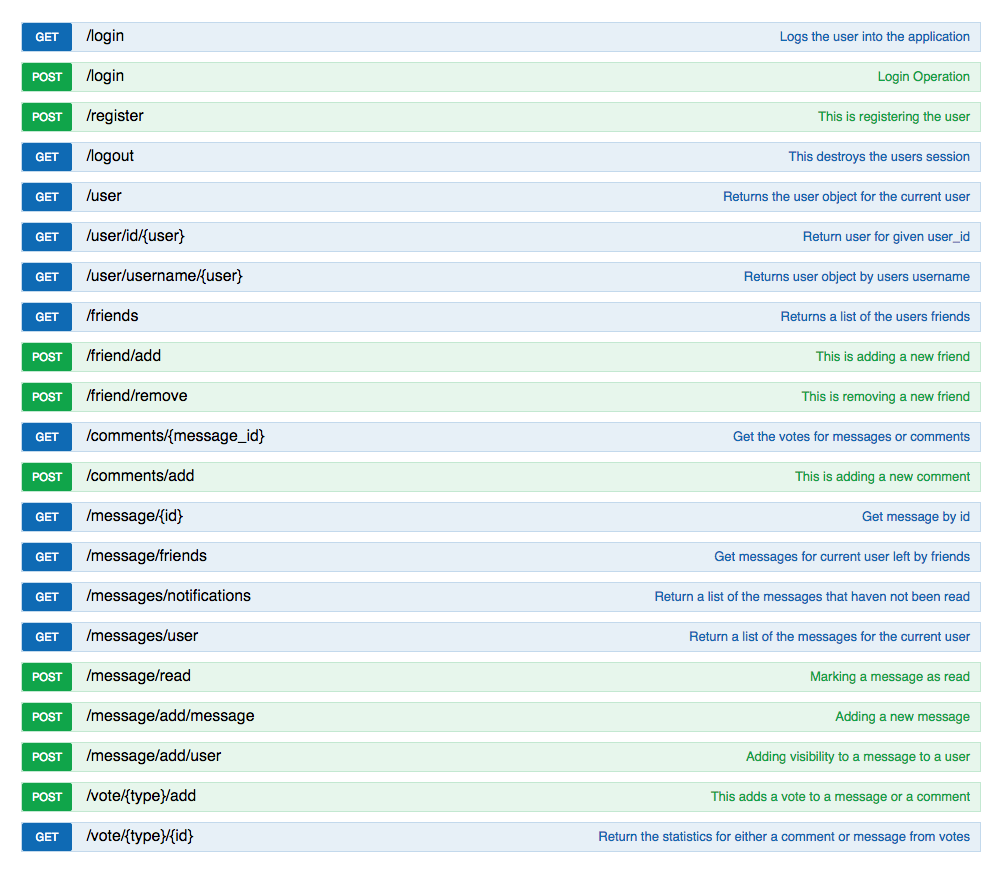
\includegraphics[width=\textwidth]{diagrams/restinterface}
    \caption{These are the endpoints for the REST API}
    \label{fig:rest_pai_diagram_image}
\end{figure} 

\subsubsection*{Structure of application}

The structure of the application is detailed within figure \ref{fig:middle_tier_code}, it has a very simple structure for the main part of the application comprising of the main deployment layer that is statically loaded code which sets up the configuration for the database \& HAPI.js server, the objects that support them are then passed to the route loader that loads the routes code dynamically that allow the application to perform its functional requirements.\\
\\
Each of the dynamically loaded modules is passed the shared object contains the references to the HAPI.js server object and to the database connector, which makes them easily accessible within the dynamically loaded code, each of the routes that are loaded dynamically loaded has its own database connector to enable a somewhat like Model View Controller type of approach to how the classes are structured, the route can call the database connector directly to get the information that is related to its various RESTful API end points that the route services. It has been on purposely done this way to ensure that to ensure flexibility within the application and enable the application to be easily extended without the need to change the main structure of the application to make the new functionality work.\\
\\
More critical parts of the application are statically loaded for example the code that deals with authenticating the user is statically loaded at the begging of authentication to ensure that it is robust and cant be tamped with once it has been loaded. For authentication it is felt that it should be a core part of the design and should be taken with up most respect and should be reasonably well engineered to ensure that the security of the application is not compromised.
 
\begin{figure}[H]
    \centering
    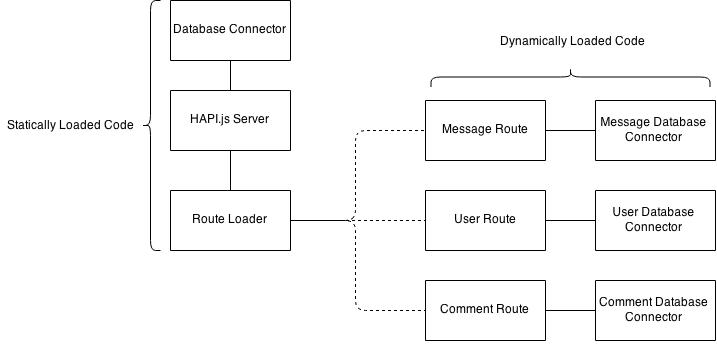
\includegraphics[width=\textwidth]{diagrams/middletier}
    \caption{Detailed structure of middle tier code}
    \label{fig:middle_tier_code}
\end{figure} 

\subsubsection*{Authentication}

The authentication procedure for the application is to used a mixed approach to authenticating the user to use the application, the user must first authenticate them selfs with basic authentication to the server which creates a session for the user and returns a cookie to them, from here the user must the cookie to authenticate them selfs against the API. HAPI.js's handles most of the background tasks for the authentication using some extra modules HAPI-Auth-Basic \& HAPI-Auth-Cookie the hook into the standard configuration to give the extra functionality that is needed for the authentication services, the code that authenticates the users is spread between the HAPI.js application and the database and has been linked together by my own development. More details about the database side of the authentication can be found in section \ref{sec:database_security}.\\
\\
This way of authenticating the user will replaced in the further development that will take place with a better standard for securing the user the use of oauth would be a much more desirable way of authenticating the user to use the middle tier services that the current method of authenticating them, at the time it was implemented into the project the current security was only there as a temporary measure for making the development secure and if time constrains had not be so tight the authentication procedure would of been upgraded to use oauth and a full review of the security procedures would be taken.

\subsection{Database level}

The database level of the application is responsible for creating a persistent store for the data that is created by the users, and making it easy to create links between the data that has been stored. In essence the database does most of the work for the application linking the various data sources together and processing it to give the application all of the its functionality that is needed to make the application work in the way specified by the functional requirements.\\
\\
It is much more efficient to get the database to process the data rather than making the middle tier do the processing work, database engines are very good at processing large amounts of data and creating links between the different types of data that are stored within the database. A database is perfect for storing large amounts of data that needs to be processed quickly and efficiently.\\
\\
It was decided that a SQL based database would be the best way of keeping and linking data together quickly efficiently behind the scenes to give the application the robust and enterprise level feel that is needed for managing and storing data. One of the more advanced features of a database is to allow robust contains to be applied to the data and ensure the data is valid for use within the application.

\subsubsection*{Choice of Technologies}
\label{sec:database_choice_of_tech}
 
It was quite straight forward decision to decide that a SQL based database was the best way forward due to its flexibility and I as a developer have a strong prior knowledge of SQL database's from working for one of the leading database experts Oracle. This was weighed up with learning a new technology the other possible choice was to go with a noSQL type database but due to the complexity of the project it was best to stick with a technology that was already known. Most of the comparison for deciding which platform to use came from Digital Oceans blog post on comparing relational database management systems \ref{ostezer:sqlframeworks:2014:online}.\\
\\
The next decision was to decide what database platform the application would be developed on there was a couple of choices for this MySQL, SQLite and PostgeSQL. SQLite was disregarded very quickly in the investigations as it is meant for much more simplistic applications and would only server an application with a max of 300 users before it would not be able to scale correctly, this is mostly down to the fact that SQLite is intended to be very simple to implement so that it can be used within embedded situations, its main benefit over the other databases is that it is highly portable and does not require large configuration to get it working correctly and would be something that could be a possible to use for caching requests on the client side application to help speed up the Android application.\\
\\
MySQL was the next on the list of platforms to research this would seem a good choice for a small to medium sized project with plenty of flexibility, it gives more advanced features than SQLite with the ability to create database functions to carry out more complicated of tasks, it offers high security features unlike SQLite as it is a custom solution it is highly customisable and can be adapted to work for any given job. Downsides is that it is not fully compliant to the SQL standard it is also missing some more advanced features that are offered by other database engines.\\
\\
The final option that was consider is PostgreSQL it offers a very advanced database engine with advanced features not offered by the other offerings and its main goal is to be standards compliant, it is well known for its data integrity capabilities. PostgresSQL is known for working well with large designs and has better integration than other solutions and rivals some propriety solutions on this matter. Some of the downsides of using PostgreSQL is that it is not very portable it is hard to configure and setup correctly along with being difficult to replicate without spending alot of time ensuring that everything is the same between the two different databases. It also has slower performance compared to some of the other solutions mentioned previously as it is not optimised for exclusively read operations from the database like for example SQLite.\\
\\
Some of the reasons PostgreSQL was chosen for this project were the advanced security features that are offered within expansions, the mature and flexible database functions offered. Probably the most important was the ability to dynamically import JSON objects directly into the database which should simplify working with the RESTful API that we are using within the middle tier as the objects that deals with specifically are all JSON objects and being to directly inject them into the database without manipulation is a very useful feature. 

\subsubsection*{Database structure}

The structure of the database has been designed around the types of data that needed to be stored for the functional requirements of the application to be for filled, the origin of the design was to store the information of the users in a secure and effective manor the focus then moved to on how messages would be stored will all the relevant fields.\\
\\
Next the biggest priority was to ensure that the messages were viewable by the persons friends so the friends section of the database was developed, after this all the auxiliary parts of the application were added this includes the comments and voting sections of the database. The design of the database grew evolutionary style to ensure that all parts were covered for the most part the design was done upfront and then morphed as the development continued.\\
\\
The figure \ref{fig:diagram_database_image} shows the connections between all of the classes and the fields held within each table, looking at this diagram it would appear that user\_id is a very commonly used field within the database which may cause issues in the future as the users table will be the table that will take the most number of requests and this data may need to be de-centralised at some point in the future as it may become a bottleneck in future, intelligent use of indexing and caching may help to prevent issues with this though. One shortcomming in the current design is there no way for there to be pending friends request for users so they will automatically come friends at the current moment the second a request is sent.

\begin{figure}[H]
    \centering
    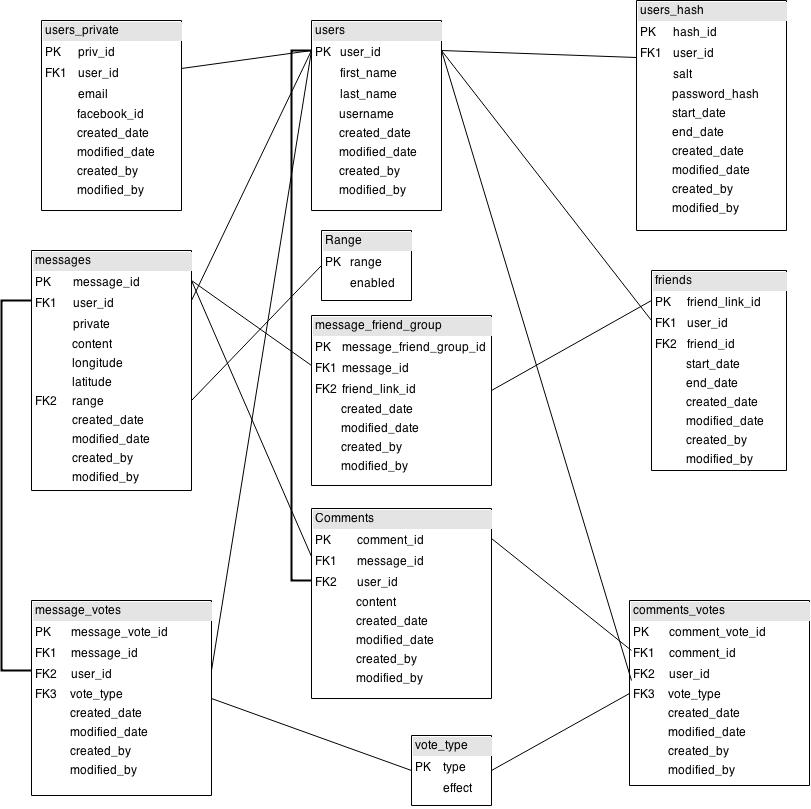
\includegraphics[width=\textwidth]{diagrams/database}
    \caption{This is the database design for the application}
    \label{fig:diagram_database_image}
\end{figure} 

\subsubsection*{Alterations}

The design had to be modified during the implementation of the project, it was mostly to ensure that the database contained all of the relevant data needed to for fill the functional requirements of the project, A later addition to the design was the ability to vote and add comments to messages. The constraints on the tables were added as the project proceeded to ensure that only correct data was entered into the database.\\
\\
One further alteration that will need to be made before the database can be used within a production environment is to add in indexing for the most important columns within the application, indexing them should help improve the performance of the database and ensure than most regularly accessed data is easy to access and is quickly indexed.\\
\\
There will need to be the ability to audit the data as well and this will also be added before the application goes into a full production, this should ensure if there are any issues then they can be traced to where it originates.

\subsubsection*{Protecting secrets}
\label{sec:database_security}

There has careful consideration taken to how sensitive data is stored within the database, the most primitive of the steps taken to help protect the users data was to separate the users data into levels of sensitivity, with the users email address and social media account id's stored away in a separate table to the main users details and there password hashes also kept in a completely different table to the rest of the users data.\\
\\
All actions to do with the users password is processed by the database engine its self, the functions that process to ensure the password is valid are kept within the database and return a status back to the middle tier to tell that the users credentials are valid so there is no chance of of sensitive data being leaked into the middle tier application.\\
\\
The users password is not stored in anyway, a MD5 of the users password is encrypted with an random encryption key which is stored along side the password this should help prevent rainbow attacks on the data left within the database and adds a extra layer of security against the possibility of compromising the data contained within the database.\\
\\
When the application is placed into the public domain steps will be made to improve the security of the data to ensure that no sensitive user data is leaked into the logs or the public domain. Currently the application uses a mixture of blowfish and MD5 to generate the salt and encryption keys that are used to protect the secrets in the application, the use of SHA-2 would be a much better hashing algorithm to use to protect the users data and will be reviewed and implemented in further development.

